\documentclass{beamer}

\usepackage{alltt}%
\usetheme{Boadilla}
\usecolortheme{seahorse}

%\usepackage{listings}
\makeatletter
\def\maxwidth{ %
  \ifdim\Gin@nat@width>\linewidth
    \linewidth
  \else
    \Gin@nat@width
  \fi
}
\makeatother

\definecolor{fgcolor}{rgb}{0.345, 0.345, 0.345}
\newcommand{\hlnum}[1]{\textcolor[rgb]{0.686,0.059,0.569}{#1}}%
\newcommand{\hlstr}[1]{\textcolor[rgb]{0.192,0.494,0.8}{#1}}%
\newcommand{\hlcom}[1]{\textcolor[rgb]{0.678,0.584,0.686}{\textit{#1}}}%
\newcommand{\hlopt}[1]{\textcolor[rgb]{0,0,0}{#1}}%
\newcommand{\hlstd}[1]{\textcolor[rgb]{0.345,0.345,0.345}{#1}}%
\newcommand{\hlkwa}[1]{\textcolor[rgb]{0.161,0.373,0.58}{\textbf{#1}}}%
\newcommand{\hlkwb}[1]{\textcolor[rgb]{0.69,0.353,0.396}{#1}}%
\newcommand{\hlkwc}[1]{\textcolor[rgb]{0.333,0.667,0.333}{#1}}%
\newcommand{\hlkwd}[1]{\textcolor[rgb]{0.737,0.353,0.396}{\textbf{#1}}}%
\let\hlipl\hlkwb

\usepackage{framed}
\makeatletter
\newenvironment{kframe}{%
 \def\at@end@of@kframe{}%
 \ifinner\ifhmode%
  \def\at@end@of@kframe{\end{minipage}}%
  \begin{minipage}{\columnwidth}%
 \fi\fi%
 \def\FrameCommand##1{\hskip\@totalleftmargin \hskip-\fboxsep
 \colorbox{shadecolor}{##1}\hskip-\fboxsep
     % There is no \\@totalrightmargin, so:
     \hskip-\linewidth \hskip-\@totalleftmargin \hskip\columnwidth}%
 \MakeFramed {\advance\hsize-\width
   \@totalleftmargin\z@ \linewidth\hsize
   \@setminipage}}%
 {\par\unskip\endMakeFramed%
 \at@end@of@kframe}
\makeatother

\definecolor{shadecolor}{rgb}{.97, .97, .97}
\definecolor{messagecolor}{rgb}{0, 0, 0}
\definecolor{warningcolor}{rgb}{1, 0, 1}
\definecolor{errorcolor}{rgb}{1, 0, 0}
\newenvironment{knitrout}{}{} % an empty environment to be redefined in TeX


\usepackage[utf8]{inputenc}
\usepackage{default}

\usepackage{xcolor}%for color mixing

\usepackage{amsmath}%
\usepackage{amsfonts}%
\usepackage{amssymb}%
\usepackage{graphicx}

\usepackage{tikz}
\usepackage{multirow}
\usepackage{booktabs}

\setbeamertemplate{itemize/enumerate body begin}{\small}

%%%%%%%%%%%%%%%%%%%%%%%%%%%%%%%%%%%%%%%%%%%%%%%%%%%%%%%%%%%%%%%%%%%%%%%%%%%%%%%%%%

\title{Linear mixed models 2}
\subtitle{Uncertainty in random effects / random interactions}
\author{Timoth\'ee Bonnet}
\date{\today}

\begin{document}

%\lstset{language=R}%code

\AtBeginSection[]
{
  \begin{frame}<beamer>
    \frametitle{}
    \tableofcontents[currentsection,sectionstyle=show/show,subsectionstyle=show/shaded/hide]% down vote\tableofcontents[currentsection,currentsubsection,hideothersubsections,sectionstyle=show/hide,subsectionstyle=show/shaded/hide] 
  \end{frame}
}

\begin{frame}{When to use random effects? Ben Bolker says:}

 \textbf{ Philosophically:}
    \small
We are not interested in the estimates of the random effects. In frequentist settings, we don’t even call these “estimates”, but rather
“predictions”, as in BLUP (best linear unbiased predictor). We want random effect levels to be drawn from a larger population, to be “exchangeable” (i.e. we could relabel/swap around the levels
without any change in meaning) and their estimates are a random variable.
%\end{block}

\textbf{Pragmatically:}
We have lots of levels, with not much information about each individual
level, and possibly unbalanced amounts of information. We don’t want to use up the degrees of freedom associated with fitting one
parameter for each level; automatically adjust between “completely pooled” (no effect) and “completely separate” (fixed effect). We have enough levels that it is practical to estimate a variance (i.e. at
least 5-6, preferably more than that).

\textbf{To Bayesians}, the difference between fixed and random is much simpler and more pragmatic: do we add a hyperparameter to the model to characterize the estimates (= random effect = we estimate a variance), or estimate them separately (= fixed effect = we use an infinite variance)?
%\end{block}

 
\end{frame}
%%%%%%%

%%%%%%%%%%%%%%%%%%%%%%%

\begin{frame}{}
\maketitle

\end{frame}
%%%%%%%%%%%%%%%%%%%%%%%


\begin{frame}{Mixed models reminder}
\centering
    \only<1>{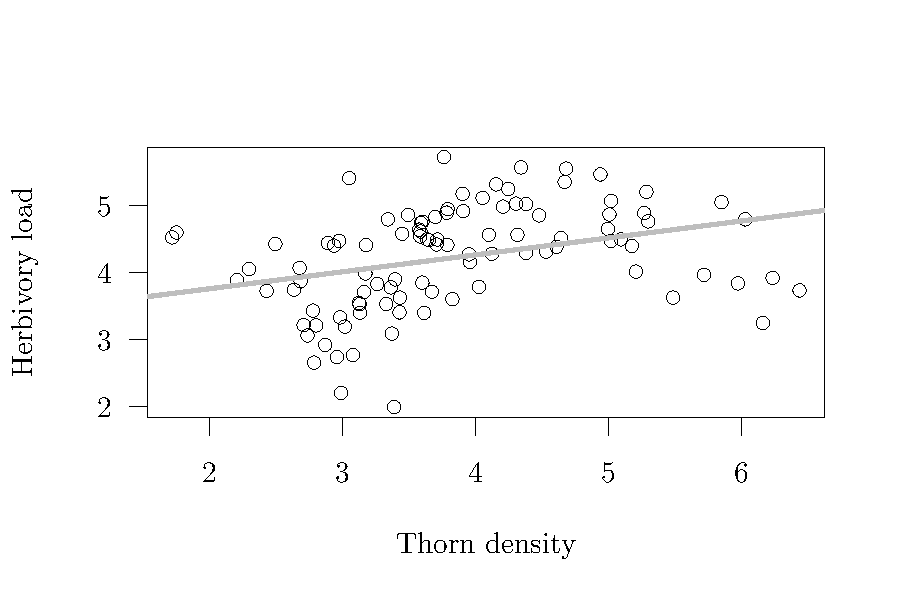
\includegraphics[width=0.9\textwidth]{figure/graph0-1}}
    \only<2>{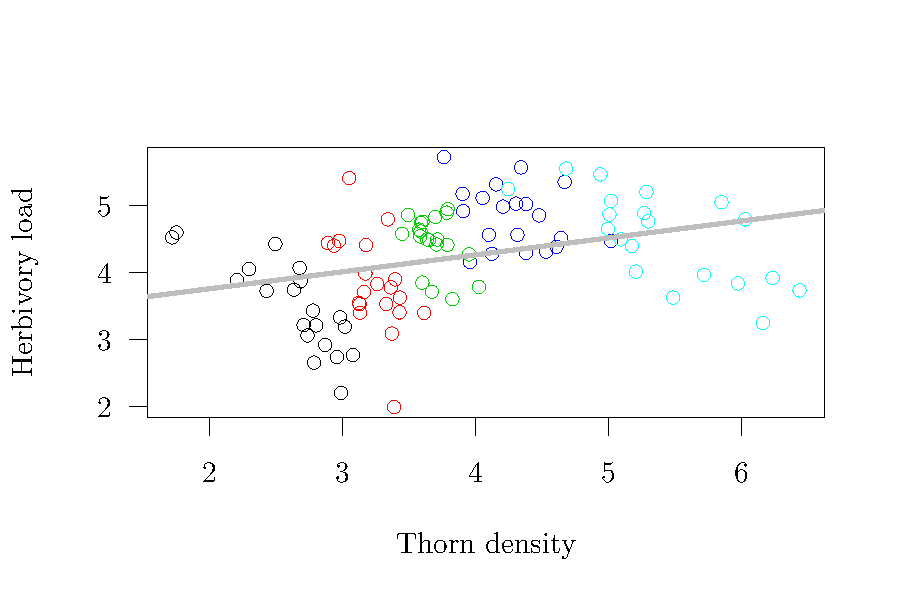
\includegraphics[width=0.9\textwidth]{figure/graph1-1}}
    \only<3>{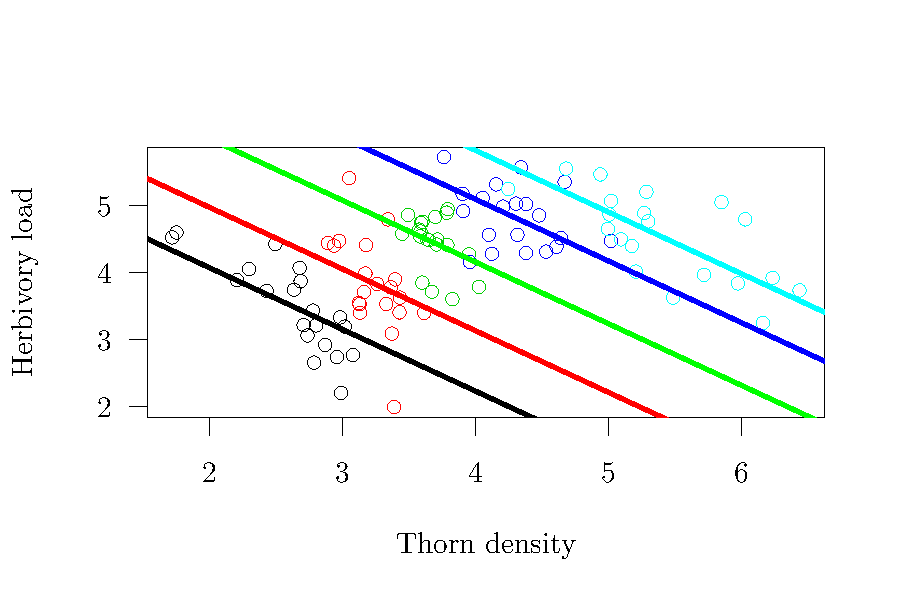
\includegraphics[width=0.9\textwidth]{figure/graph2-1}}
\end{frame}
%%%%%%%%%%%
\begin{frame}{Mixed models reminder}
\vspace{-1cm}
\begin{columns}
    \begin{column}{0.5\textwidth}
     1. First model assumes residuals are independent\\
     \vspace{1cm}
     2. But they are not. Data come from five different places\\
     \vspace{1cm}
     
     3. Adding random effect ``place'' gets correct slope. Residuals are now really independent
    \end{column}

    \begin{column}{0.5\textwidth}
     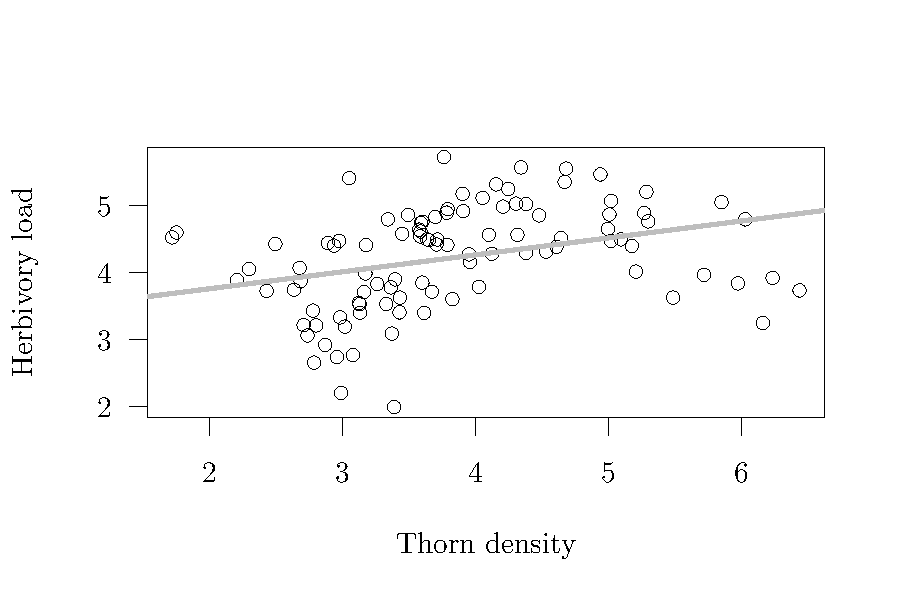
\includegraphics[width=0.9\textwidth]{figure/graph0-1}\vspace{-1cm}
     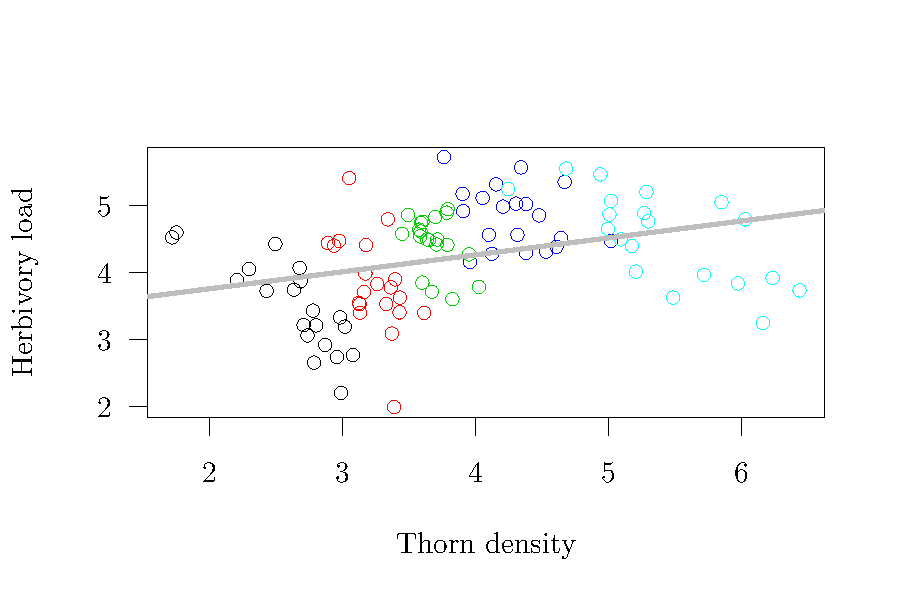
\includegraphics[width=0.9\textwidth]{figure/graph1-1}\vspace{-1cm}
     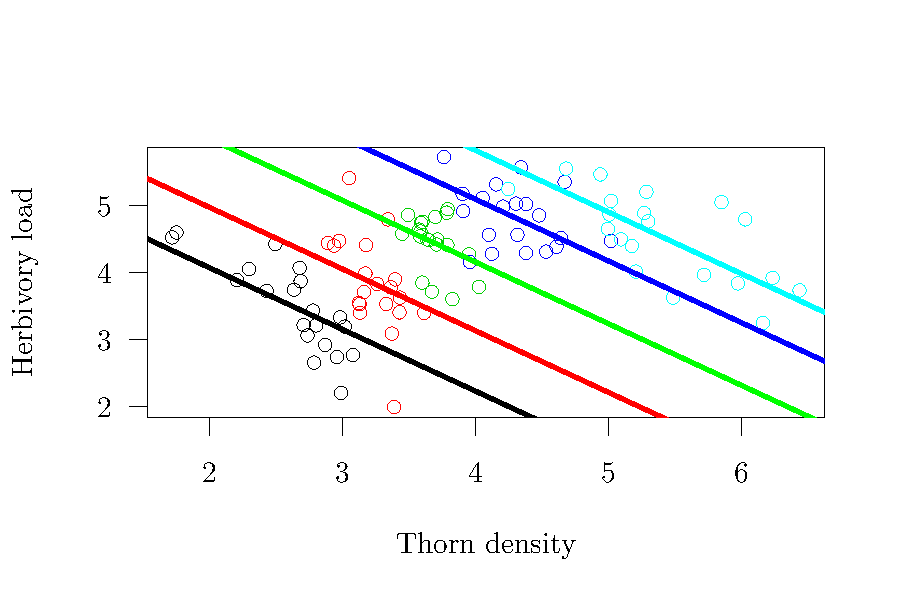
\includegraphics[width=0.9\textwidth]{figure/graph2-1}
    \end{column}
\end{columns}

\end{frame}
%%%%%%%%%%%

\begin{frame}{Mixed models reminder}
\textbf{Add a random effect to a basic lm:\\}

\texttt{lm(response $\sim$ predictor, data=thorns)}\\

\texttt{library(lme4)}\\
\texttt{lmer(response $\sim$ predictor + (1|block), data=thorns)}\\


\vfill
\only<2>{\large \color{blue} \textbf{Demo in R: Excercise 1}}

\only<3->{
\begin{alertblock}{Questions you may have:}
    \begin{itemize}
     \item Is the random effect ``significant''?
     \item Should I include as many random effects as possible?
    \end{itemize}
\end{alertblock}}

\end{frame}
%%%%%%%%%

\begin{frame}{Mixed models today}
 
 \begin{enumerate}
 \large
  \item Quantify uncertainty in random effects
    \begin{itemize}
     \item p-values and tests (\textit{R-coding!})
     \item confidence intervals
     \item BLUPs = random effect levels
    \end{itemize}
  \item Beyond random intercepts
    \begin{itemize}
     \item Random interactions
    \end{itemize}

 \end{enumerate}
 

\end{frame}
%%%%%%%%%%%

\section{Uncertainty in random effects}

\begin{frame}{Uncertainty in random effects}
 
 \texttt{lmm1 <- lmer(herbivory $\sim$ thorndensity + (1|site), data=thorns)}\\
 \texttt{summary(lmm1)}\\
 
Does not measure uncertainty in site variance. Does ``site'' matter?
 
 \pause
 \begin{exampleblock}{How to?}
 \begin{itemize}
  \item Confidence interval: far from zero? How does it compare to residual variance or total variance?
  \item Null-hypothesis testing: p-value.
 \end{itemize}
 \textbf{Exercises 2 and 3}
\end{exampleblock}
\end{frame}
%%%%%%%

\begin{frame}{Issue with null-hypothesis testing for random effects}
 
 \textbf{What is a p-value?}\\
 \pause
 \textbf{How do we know whether a test works?}\\
 
 \pause
 \vfill
 \textbf{Let's check with \color{blue} Exercise 4}
\end{frame}
%%%%%%%

\begin{frame}{Issue with null-hypothesis testing for random effects}
\begin{alertblock}{Why??}
    A variance cannot be negative. Anova doesn't know.\\
    P-value computed as \texttt{1-pchisq(LRT0\$Chisq[2],df=1)} but there is LESS than one degree of freedom.
\end{alertblock}
\pause
\begin{exampleblock}{Solutions, from worse to best:}
    \begin{itemize}
     \item Acknowledge test is conservative (i.e., too rarely significant) 
     \item Divide p-value by 2
     \item Use half a degree of freedom \texttt{1-pchisq(LRT0\$Chisq[2],df=0.5)} 
    \end{itemize}

\end{exampleblock}

\pause
NB: same problem with AIC, a random intercept should maybe count as 0.5 parameter, but R always count 1 parameter. Actually it is more complicated and there is no definitive answer yet! 

\end{frame}
%%%%%%%

\begin{frame}{Example of application: repeatability}
 Do kangaroos have personality = repeatable behaviour?\\(inspired by Weliton's work)
 \begin{figure}
 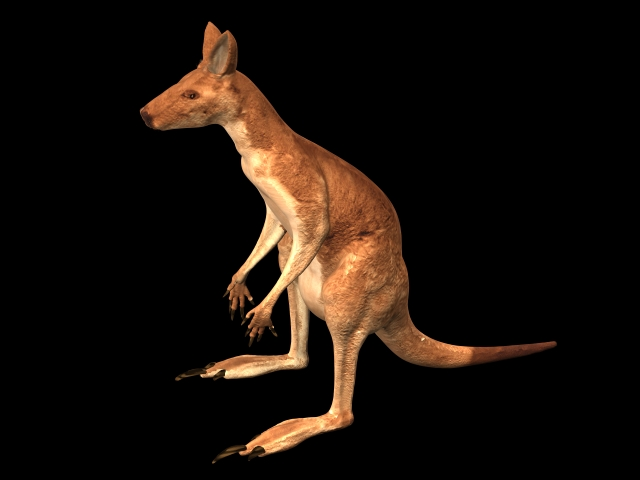
\includegraphics[width=0.5\textwidth]{figure/roo}
 \end{figure}
 
 
\end{frame}
%%%%%%%

%%%%%%
\begin{frame}{Should you test and remove non-significant random effects}
 
 \begin{block}{Test?}
    \begin{itemize}
     \item \textbf{Yes if effect of interest}
     \item Optional if ``nuisance'' parameter part of experimental design
    \end{itemize}
\end{block}
\pause
 \begin{block}{Remove non-significant?}
    \begin{itemize}
     \item No if clearly part of experimental design
     \item But doesn't matter if estimated variance is zero
     \item Maybe remove if model too complex (i.e., difficult to interpret or convergence issues) but acknowledge assumptions!
    \end{itemize}
\end{block}
 
\end{frame}
%%%%%%%


\section{Beyond random intercepts}

\begin{frame}{Not only intercept vary!}
\centering
    \only<1>{
    Assume parallel slopes:
    
    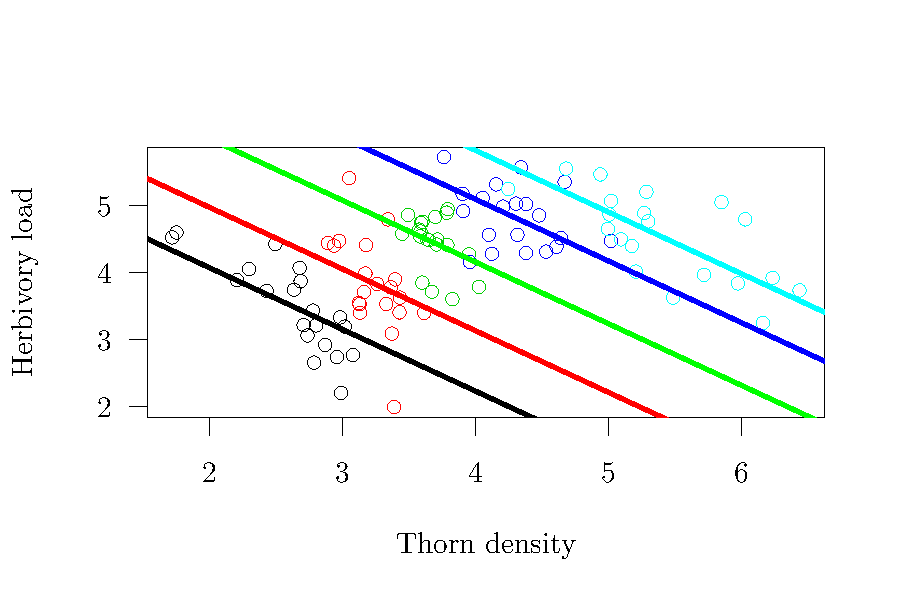
\includegraphics[width=0.9\textwidth]{figure/graph2-1}}
    \only<2>{
    Allow slopes to vary:
    
    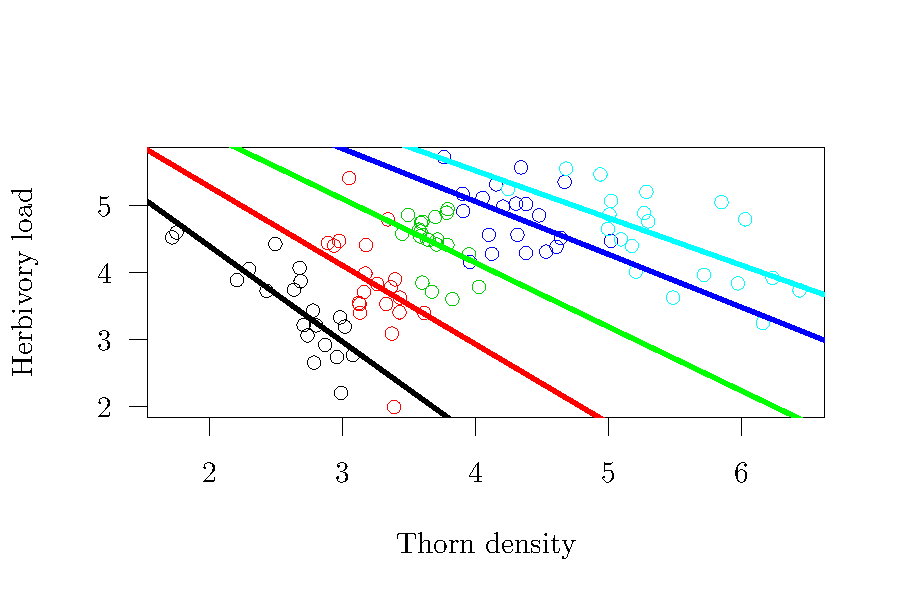
\includegraphics[width=0.9\textwidth]{figure/graphrslopes-1}}
\end{frame}
%%%%%%%

\begin{frame}{How to?}

\begin{alertblock}{Right-hand side = what groups observations}
Nested, crossed et al. on the right hand side of the \texttt{|}: \texttt{(1|something)}\\
How are data related to each other, what groups them\\
\end{alertblock}


\pause
\begin{alertblock}{\textbf{Left-hand side = what varies according to grouping}}
The \texttt{1} stands for \textbf{intercept}\\
But many things can go to the left hand side. \\
Random interactions, random regressions, random slopes\dots
 e.g., $y \sim 1 + x + (1 + x | something)$
\end{alertblock}
 
\end{frame}
%%%%%%%%%%%



\begin{frame}{Everything you need to know about mixed models}

\begin{itemize}
 \item \url{http://bbolker.github.io/mixedmodels-misc/glmmFAQ.html}
 \item Subscribe to mailing-list: \texttt{https://stat.ethz.ch/mailman/listinfo/r-sig-mixed-models}
\end{itemize}

\end{frame}
%%%%%%%%%%%%%


\end{document}
